%%%%%%%%%%%%%%%%%%%%%%%%%%%%%%%%%%%%%%%%%
% Masters/Doctoral Thesis 
% LaTeX Template
% Version 2.5 (27/8/17)
%
% This template was downloaded from:
% http://www.LaTeXTemplates.com
%
% Version 2.x major modifications by:
% Vel (vel@latextemplates.com)
%
% This template is based on a template by:
% Steve Gunn (http://users.ecs.soton.ac.uk/srg/softwaretools/document/templates/)
% Sunil Patel (http://www.sunilpatel.co.uk/thesis-template/)
%
% Template license:
% CC BY-NC-SA 3.0 (http://creativecommons.org/licenses/by-nc-sa/3.0/)
%
%%%%%%%%%%%%%%%%%%%%%%%%%%%%%%%%%%%%%%%%%

%----------------------------------------------------------------------------------------
%	PACKAGES AND OTHER DOCUMENT CONFIGURATIONS
%----------------------------------------------------------------------------------------
\documentclass[
11pt, % The default document font size, options: 10pt, 11pt, 12pt
oneside, % Two side (alternating margins) for binding by default, uncomment to switch to one side
english, % ngerman for German
singlespacing, % Single line spacing, alternatives: onehalfspacing or doublespacing
%draft, % Uncomment to enable draft mode (no pictures, no links, overfull hboxes indicated)
%nolistspacing, % If the document is onehalfspacing or doublespacing, uncomment this to set spacing in lists to single
%liststotoc, % Uncomment to add the list of figures/tables/etc to the table of contents
%toctotoc, % Uncomment to add the main table of contents to the table of contents
%parskip, % Uncomment to add space between paragraphs
%nohyperref, % Uncomment to not load the hyperref package
headsepline, % Uncomment to get a line under the header
chapterinoneline, % Uncomment to place the chapter title next to the number on one line
%consistentlayout, % Uncomment to change the layout of the declaration, abstract and acknowledgements pages to match the default layout
]{MastersDoctoralThesis} % The class file specifying the document structure

\usepackage[utf8]{inputenc} % Required for inputting international characters
\usepackage[T1]{fontenc} % Output font encoding for international characters
\usepackage{mathpazo} % Use the Palatino font by default
\usepackage{cite}

%\usepackage[backend=bibtex,style=numeric,sorting=none, maxbibnames=99]{biblatex} % Use the bibtex backend with the authoryear citation style (which resembles APA)

%\addbibresource{~/BibTex/BibTex.bib} % The filename of the bibliography

\usepackage[autostyle=true]{csquotes} % Required to generate language-dependent quotes in the bibliography

\usepackage{amstext, amsfonts, amsmath, amsbsy, amssymb}
\usepackage{tikz}
\usepackage{booktabs}
\usepackage{pgfplots}
\usepackage{caption}
\usepackage{subcaption}
\usepackage{easyReview}

%----------------------------------------------------------------------------------------
%	MARGIN SETTINGS
%----------------------------------------------------------------------------------------

\geometry{
	paper=a4paper, % Change to letterpaper for US letter
	inner=2.5cm, % Inner margin
	outer=3.8cm, % Outer margin
	bindingoffset=.5cm, % Binding offset
	top=1.5cm, % Top margin
	bottom=1.5cm, % Bottom margin
	%showframe, % Uncomment to show how the type block is set on the page
}

%----------------------------------------------------------------------------------------
%	THESIS INFORMATION
%----------------------------------------------------------------------------------------

\thesistitle{Anticipating the chemical compositions of organisms across the tree of life.} % Your thesis title, this is used in the title and abstract, print it elsewhere with \ttitle
\supervisor{Prof. Daniel \textsc{Wegmann} \\ \& Dr. Pierre-Marie \textsc{Allard}} % Your supervisor's name, this is used in the title page, print it elsewhere with \supname
\examiner{} % Your examiner's name, this is not currently used anywhere in the template, print it elsewhere with \examname
\degree{Master of Science in Bioinformatics and Computational Biology} % Your degree name, this is used in the title page and abstract, print it elsewhere with \degreename
\author{Marco \textsc{Visani}} % Your name, this is used in the title page and abstract, print it elsewhere with \authorname
\addresses{} % Your address, this is not currently used anywhere in the template, print it elsewhere with \addressname

\subject{Biological Sciences} % Your subject area, this is not currently used anywhere in the template, print it elsewhere with \subjectname
\keywords{} % Keywords for your thesis, this is not currently used anywhere in the template, print it elsewhere with \keywordnames
\university{\href{https://www.unifr.ch/}{University of Fribourg}} % Your university's name and URL, this is used in the title page and abstract, print it elsewhere with \univname
\department{\href{https://www.unifr.ch/bio/en/}{Department of Biology}} % Your department's name and URL, this is used in the title page and abstract, print it elsewhere with \deptname
\group{\href{https://www.unifr.ch/bio/en/groups/wegmann/}{Wegmann Group} \& \href{https://www.unifr.ch/bio/en/groups/allard/}{COMMONS Lab}} % Your research group's name and URL, this is used in the title page, print it elsewhere with \groupname
\faculty{\href{https://www.unifr.ch/scimed/en/}{Faculty of Science and Medicine}} % Your faculty's name and URL, this is used in the title page and abstract, print it elsewhere with \facname

\AtBeginDocument{
\hypersetup{pdftitle=\ttitle} % Set the PDF's title to your title
\hypersetup{pdfauthor=\authorname} % Set the PDF's author to your name
\hypersetup{pdfkeywords=\keywordnames} % Set the PDF's keywords to your keywords
}


%----------------------------------------------------------------------------------------
%	MATH STUFF
\usepackage{amstext, amsfonts, amsmath, amsbsy, amssymb}
\DeclareMathOperator{\Poisson}{Poisson}
\DeclareMathOperator{\Multinom}{Multinom}
\DeclareMathOperator{\logit}{logit}
\DeclareMathOperator{\cov}{cov}
\DeclareMathOperator{\Ind}{I}
\def\P{\mathbb{P}}
\def\E{\mathbb{E}}

\def\x{\boldsymbol{x}}

\def\btau{\boldsymbol{\tau}}
\def\bmu{\boldsymbol{\mu}}
\def\bxi{\boldsymbol{\xi}}
\def\bLambda{\boldsymbol{\Lambda}}
\def\bP{\boldsymbol{P}}
\def\bd{\boldsymbol{d}}


\def\Ccal{{\cal C}}
\def\E{{\cal E}}
\def\I{{\cal I}}
\def\N{{\cal N}}
\def\M{{\cal M}}
\def\R{{\cal R}}
\def\T{{\cal T}}
\def\X{{\cal X}}
\def\Y{{\cal Y}}
\def\Z{{\cal Z}}


%----------------------------------------------------------------------------------------

\linespread{1.25}
\begin{document}


\frontmatter % Use roman page numbering style (i, ii, iii, iv...) for the pre-content pages

\pagestyle{plain} % Default to the plain heading style until the thesis style is called for the body content

%----------------------------------------------------------------------------------------
%	TITLE PAGE
%----------------------------------------------------------------------------------------

\begin{titlepage}

\includegraphics[scale=0.3]{figure/UnifrLogo} % University logo
\begin{center}
\vspace*{.06\textheight}
{\scshape\LARGE \univname\par}\vspace{1.5cm} % University name

\textsc{\Large Master Thesis}\\[0.5cm] % Thesis type

\HRule \\[0.4cm] % Horizontal line
{\huge \bfseries \ttitle\par}\vspace{0.4cm} % Thesis title
\HRule \\[1.5cm] % Horizontal line
 
\begin{minipage}[t]{0.4\textwidth}
\begin{flushleft} \large
\emph{Author:}\\
\href{mailto:contact@vismarco.ch}{\authorname} % Author name - remove the \href bracket to remove the link
\end{flushleft}
\end{minipage}
\begin{minipage}[t]{0.4\textwidth}
\begin{flushright} \large
\emph{Supervisors:} \\
\href{mailto:daniel.wegmann@unifr.ch}{Prof. Daniel \textsc{Wegmann}} \\
\href{mailto:pierre-marie.allard@unifr.ch}{Dr. Pierre-Marie \textsc{Allard}}% Supervisor name - remove the \href bracket to remove the link  
\end{flushright}
\end{minipage}\\[3cm]
 
\vfill

\large \textit{A thesis submitted in fulfillment of the requirements \\ for the degree of \degreename}\\[0.3cm] % University requirement text
\textit{in the}\\[0.4cm]
\groupname\\\deptname\\[2cm] % Research group name and department name
 
\vfill

{\large \today}\\[4cm] % Date
%\includegraphics{Logo} % University/department logo - uncomment to place it
 
\vfill
\end{center}
\end{titlepage}

%----------------------------------------------------------------------------------------
%%	DECLARATION PAGE
%%----------------------------------------------------------------------------------------
%
%\begin{declaration}
%\addchaptertocentry{\authorshipname} % Add the declaration to the table of contents
%\noindent I, \authorname, declare that this thesis titled, \enquote{\ttitle} and the work presented in it are my own. I confirm that:
%
%\begin{itemize} 
%\item This work was done wholly or mainly while in candidature for a research degree at this University.
%\item Where any part of this thesis has previously been submitted for a degree or any other qualification at this University or any other institution, this has been clearly stated.
%\item Where I have consulted the published work of others, this is always clearly attributed.
%\item Where I have quoted from the work of others, the source is always given. With the exception of such quotations, this thesis is entirely my own work.
%\item I have acknowledged all main sources of help.
%\item Where the thesis is based on work done by myself jointly with others, I have made clear exactly what was done by others and what I have contributed myself.\\
%\end{itemize}
% 
%\noindent Signed:\\
%\rule[0.5em]{25em}{0.5pt} % This prints a line for the signature
% 
%\noindent Date:\\
%\rule[0.5em]{25em}{0.5pt} % This prints a line to write the date
%\end{declaration}
%
%\cleardoublepage

%----------------------------------------------------------------------------------------
%	QUOTATION PAGE
%----------------------------------------------------------------------------------------

%\vspace*{0.2\textheight}
%
%\noindent\enquote{\itshape Thanks to my solid academic training, today I can write hundreds of words on virtually any topic without possessing a shred of information, which is how I got a good job in journalism.}\bigbreak
%
%\hfill Dave Barry

%----------------------------------------------------------------------------------------
%	ABSTRACT PAGE
%----------------------------------------------------------------------------------------

\begin{abstract}\label{sec:abstract}
\addchaptertocentry{\abstractname} % Add the abstract to the table of contents
This study is centered on Natural Products (NPs) - specific chemicals synthesized by living organisms. These NPs hold significant importance in various domains, notably medicine, agriculture, and ecology. A primary resource for our research is the LOTUS database, which catalogues a vast array of NPs. Yet, a gap exists: there's no existing model to predict the occurrence of these NPs across different species.

Our research project began on a course that was initially distinguished by a traditional analytical approach. Although simple, this strategy immediately showed its shortcomings when dealing with the complex nature of Natural Products (NPs). We switched to an advanced graph-based method after seeing the necessity for a more thorough strategy to accurately represent the intricate interactions present in NPs. This development marked a fundamental evolution in our understanding and handling of the data rather than merely a change in technique. The graph-based method views data as a network of related entities, providing a far more comprehensive and in-depth viewpoint. By using this improved methodology, we have created a more fruitful path for exploring the complex world of Natural Products. We think that this strategy will open up new research directions and possibly result in ground-breaking NP-related findings.
\end{abstract}

%----------------------------------------------------------------------------------------
%	ACKNOWLEDGEMENTS
%----------------------------------------------------------------------------------------

\begin{acknowledgements}\label{sec:acknowledgements}
\addchaptertocentry{\acknowledgementname} % Add the acknowledgements to the table of contents
The acknowledgments and the people to thank go here, don't forget to include your project advisor\ldots TODO
\end{acknowledgements}

%----------------------------------------------------------------------------------------
%	LIST OF CONTENTS/FIGURES/TABLES PAGES
%----------------------------------------------------------------------------------------

\tableofcontents % Prints the main table of contents

%\listoffigures % Prints the list of figures

%\listoftables % Prints the list of tables

%----------------------------------------------------------------------------------------
%	ABBREVIATIONS
%----------------------------------------------------------------------------------------
%
\begin{abbreviations}{ll}\label{sec:abbreviations} % Include a list of abbreviations (a table of two columns)
	
\textbf{CC}  & \textbf{C}ollective \textbf{C}lassification \\
\textbf{DAG} & \textbf{D}irected \textbf{A}cyclic \textbf{G}raph\\
\textbf{GCN(s)} & \textbf{G}raph \textbf{C}onvolutional \textbf{N}etwork(s) \\
\textbf{GNN(s)} & \textbf{G}raph \textbf{N}eural \textbf{N}etwork(s) \\
\textbf{(k)PCA} & (kernel) \textbf{P}rincipal \textbf{C}omponent \textbf{A}nalysis \\
\textbf{MS} & \textbf{M}ass \textbf{S}pectrometry \\
\textbf{NP(s)} & \textbf{N}atural \textbf{P}roduct(s) \\
\textbf{RMF} & \textbf{R}andom \textbf{M}arkov \textbf{F}ield \\



\end{abbreviations}

%----------------------------------------------------------------------------------------
%	PHYSICAL CONSTANTS/OTHER DEFINITIONS
%----------------------------------------------------------------------------------------

%\begin{constants}{lr@{${}={}$}l} % The list of physical constants is a three column table
%
%% The \SI{}{} command is provided by the siunitx package, see its documentation for instructions on how to use it
%
%Speed of Light & $c_{0}$ & \SI{2.99792458e8}{\meter\per\second} (exact)\\
%%Constant Name & $Symbol$ & $Constant Value$ with units\\
%
%\end{constants}

%----------------------------------------------------------------------------------------
%	SYMBOLS
%----------------------------------------------------------------------------------------

%\begin{symbols}{lll}\label{sec:symbols} % Include a list of Symbols (a three column table)
%
%$a$ & distance & \si{\meter} \\
%$P$ & power & \si{\watt} (\si{\joule\per\second}) \\
%%Symbol & Name & Unit \\
%
%\addlinespace % Gap to separate the Roman symbols from the Greek
%
%$\omega$ & angular frequency & \si{\radian} \\
%
%\end{symbols}

%----------------------------------------------------------------------------------------
%	DEDICATION
%----------------------------------------------------------------------------------------

%\dedicatory{For/Dedicated to/To my\ldots} 

%----------------------------------------------------------------------------------------
%	THESIS CONTENT - CHAPTERS
%----------------------------------------------------------------------------------------

\mainmatter % Begin numeric (1,2,3...) page numbering

\pagestyle{thesis} % Return the page headers back to the "thesis" style

% Include the chapters of the thesis as separate files from the Chapters folder
% Uncomment the lines as you write the chapters

%\include{Chapters/1_introduction}
%\include{Chapters/2_litterature_review} 
%\include{Chapters/3_methods}
%\include{Chapters/4_results} 
%\include{Chapters/5_discussion} 
%\include{Chapters/6_conclusion}

\chapter{Introduction}\label{chap:intro}

\section{Natural Products: Definition and Roles}\label{sec:NP def and roles}
Natural Products (NPs) are chemical entities biosynthesized by living organisms \cite{AllNatural2007}. Numerous NPs are metabolites, which can be arranged along a gradient of specialisation from core metabolites, which perform fundamental tasks and are present in a variety of organisms, to specialised metabolites, which are much more restricted across the tree of life. A transdisciplinary area, natural product research is interested in the underlying structural features of naturally occurring molecular entities, their effects on living things, and even the study of chemically mediated interactions across entire ecosystems. We will use \textit{Rutz et al.}'s in definition of Natural Product \textit{as any chemical entity found in a living organism}, \textit{i.e.} a structure-organism pair \cite{rutzLOTUSInitiativeOpen2022}.

\section{The Importance of Natural Products in Therapeutics and Ecosystem Functioning}
Specialised metabolites form the basis of current therapeutic treatments because of their distinct chemical structures and activities \cite{harveyReemergenceNaturalProducts2015}. They are relevant to a variety of industries, including agriculture \cite{yanImpactProspectNatural2018}, the food industry \cite{gonzalez-manzanoApplicationsNaturalProducts2021}, cosmetics \cite{liuNaturalProductsCosmetics2022}, and a variety of other fields, in addition to human and veterinary medicine. These natural goods are inextricably related to renewable resources and add great value in our economy.

Understanding the complexities of their biological functions and structural characteristics is essential to understanding how ecosystems work. These complexities influence a variety of aspects, from the impact on individual organisms to the overall chemically mediated interactions within the entire ecosystem.

Numerous fundamental scientific ideas, such as stereochemistry, optical activity, regioselectivity, and chirality, have also been influenced by natural products. Researchers are always motivated by their diversity and complexity, which leads to the development of cutting-edge tools that can replicate natural processes to manage bioregulation mechanisms and solve practical problems  \cite{drasarGrowingImportanceNatural2019}.

Even though they're complex and challenging to describe, the role of natural products in therapeutic uses and ecosystem functionality cannot be overstated. Current developments aim to unlock this potential more efficiently, emphasizing the ongoing advancements across all sectors associated with natural products.

\section{The LOTUS Database and Current Efforts}
In recent years, efforts have been made to anticipate metabolic networks or occurrences of molecules in selected taxa. A significant resource is the LOTUS database \cite{rutzLOTUSInitiativeOpen2022} developed and maintained by the \href{https://www.unifr.ch/bio/en/groups/allard/}{COMMONS lab}, which currently lists over 438'072 occurrences of natural products in selected taxa. The LOTUS initiative aims to consolidate and share structure-organism pair information via an open platform, providing transformative potential for natural products research and beyond. This process involves the harmonization, curation, validation, and open dissemination of referenced structure-organism pairs. Furthermore, LOTUS data's embedding into the vast Wikidata knowledge graph facilitates new biological and chemical insights. The contemporary bioinformatic capabilities offered by the LOTUS initiative have the potential to reshape knowledge management, analysis, and interpretation of data in natural products research. Despite this, no model has been proposed to predict occurrence of structure-organism pairs across the tree of life.

\section{Project Description and Objectives}
The goal of this project is to develop such a model and to train it using large-scale metabolomics and other occurrence data.

For this research, we consider two primary sources of information : 1) The LOTUS database, which catalogues presence-only attestations of discrete metabolites inherent to specific taxa, as corroborated by peer-reviewed scientific literature. 2) Data derived from mass spectrometry (MS) analyses.

The strict data integrity of LOTUS is what gives it its inherent value. This is mainly attributable to the actual extraction and characterization of chemicals from particular living entities, which guarantees unmatched data authenticity. Despite its accuracy, the methodological framework supporting LOTUS requires a lot of effort and resources. Currently, just 0.008\% of all potential occurrences in the database are represented by the 438,072 occurrences that have been archived in LOTUS. A thorough knowledge of the genuine presence or absence matrix of molecules across the evolutionary spectrum is still difficult given the pace of academic research.

In contrast, mass spectrometry (MS) provides a quicker and more practical approach of molecular detection. However, this increased effectiveness comes with built-in restrictions. In particular, MS shows limitations when trying to identify molecules with previously unidentified structural configurations. Furthermore, when compared to techniques that rely on actual molecule separation, MS's resolution and fidelity are noticeably reduced; in contrast, the latter need careful compound extraction and characterisation, whereas MS primarily function as a detection mechanism.

By integrating these two sources of information and using an appropriate model, it may be feasible to anticipate the complete chemical composition of organisms across the tree of life. 


%\chapter{Literature Review}


\chapter{Theoretical introduction}\label{chap:Theoretical introduction}
A graph is a collection of elements, known as vertices or nodes, and their connections, known as edges or links, in the world of mathematical structures. Edges represent the connections or affiliations between pairs of these points, whilst vertices serve as discrete points or units. For example, in biology, a graph can show the complex network of connections between proteins in a cellular system. Each protein is represented by a node, and the functional or physical relationships between them are denoted by edges \cite{trudeauIntroductionGraphTheory1993}. 

Often, these nodes carry specific attributes. In our work, these might include attributes such as the molecule's atomic structure, size, or charge. However, the acquisition of comprehensive attribute data can be challenging due to obstacles in data collection, inherent complexity, or, in some cases, privacy concerns. To mitigate this, graph-based semi-supervised learning, also known as node classification, is employed to predict missing attributes (i.e., labels y) for some nodes given known attributes (i.e., features x). This strategy has been effective in a myriad of applications, including predicting molecular functions and categorization of substances \cite{NIPS2016_390e9825, liDeeperInsightsGraph2018}.

Link prediction is a fundamental task in graph theory, aiming to forecast the likelihood of a potential relationship or edge between two nodes within a network. In the context of social networks, as highlighted by Liben-Nowell and Kleinberg \cite{liben-nowellLinkPredictionProblem2003}, the challenge is to determine which interactions are likely to emerge in the future based on the current network topology. The underlying hypothesis is that the inherent structure of the network contains valuable information about future interactions. Various measures of node "proximity" or similarity within the network can be employed to make these predictions, and some nuanced measures have been found to outperform more direct ones \cite{zhangLinkPredictionBased2018}.

Graph neural networks (GNNs) \cite{wuGraphNeuralNetworks2022} have been frequently employed for semi-supervised learning or for link predictions, also in the context of molecular networks \cite{oyetundeBoostGAPFILLImprovingFidelity2017}. Initially, GNNs synthesize the features and graph structure in the vicinity of each node into a single vector representation. Subsequently, this representation is individually used for the classification of each node. The benefits of using GNNs include automatic differentiation enabling end-to-end training and straightforward sub-sampling schemes for handling extensive networks. However, the use of GNNs hinges on the assumption that node labels are conditionally independent given all features. Moreover, these networks do not leverage correlations between training and testing labels during inference, and due to the complexities of their transformations and aggregation functions, the derived models can be challenging to interpret.

Alternatively, collective classification (CC) \cite{senCollectiveClassificationNetwork2008} provides an interpretable approach, utilizing graphical models that directly exploit label correlation for prediction. One such model used within our research is Markov networks also known as Markov random field (RMF). RMFs model the joint distribution of all node labels within a conditional random field and predict an unknown label with its marginal probabilities. This method allows for the leveraging of label correlation during inference, which involves conditioning on the training labels. However, the increased interpretability and convenience of collective classification come at a price. The models are learned by maximizing the joint likelihood, rendering end-to-end training extremely difficult. This, in turn, restricts the capacity and versatility of the model \cite{jiaGraphBeliefPropagation2021}.

Our research did not initially utilize a graph-based approach. We started our work using more traditional, naive methods that treated our data as a simple collection of independent observations rather than recognizing the inherent interconnectedness of the molecular structures and interactions within organisms. This initial approach, while more straightforward, failed to fully capture the intricate complexity and interconnected nature of our dataset, a key characteristic of biological systems.

However, recognizing the limitations of such naive methods, we transitioned to the use of graphical models, specifically graph neural networks and collective classification techniques. This shift in our modelling paradigm has significantly enhanced our ability to predict the molecules present in any organism on Earth, allowing for the more effective use of both the Markov random field approach and GNNs. By treating our data as a graph, we've been better equipped to capture the nuanced relationships and dependencies between different molecular entities and their attributes.

\section{Naive approach}\label{sec:methods:Naive approach}
Our objective is to infer the occurrence or absence of metabolites across a collection of samples, which are differentiated by $T$ discrete dimensions such as species, tissue type, and environmental conditions or any other arbitrary dimension. For any compartment $c$, let $\tau_t(c) = 1, \ldots, n_t$ indicate the compartment index along axis $t=1, \ldots, T$. For convenience, let us further denote by $\tau_\M(c)$ and $\tau_\S(c)$ the metabolite and species of that compartment.

We denote $x_{c}$ the presence ($x_c=1$) or absence ($x_c=0$) of a metabolite $\tau_\M(c)$ in compartment $c$ and let $\x=(x_1, \ldots, x_C)$ be the full vector $x_c$ across all compartments $c=1, \ldots, C$ with $C=\prod_t n_t$.

We will assume that similarities across any of the axes of compartmentalization is reflected in the patterns of presences and absences in $\x$. For instance, closely related species may share a similar set of metabolites and  metabolites related in their synthesis may share a similar distribution across species. To model such similarities, we assume that the probability $\P(x_c=1|\bmu_c, \epsilon_c)$ with which metabolite $\tau_\M(c)$ is present in compartment $c$ is given by

\begin{equation}\label{eq:logit of X}
	\logit \P(x_c=1|\bmu_c, \epsilon_c) = \sum_{t=1}^{T} \mu^{(t)}_{\tau_t(c)} + \epsilon_{c}
\end{equation}

where $\bmu_c=(\mu^{(1)}_{\tau_1(c)}, \ldots, \mu^{(T)}_{\tau_T(c)})$ is a vector of axis specific intercepts and $\epsilon_{c}$ is normally distributed with mean 0 and co-variance

\begin{equation}
	\cov(\epsilon_c, \epsilon_{c'}) = \sum_t \beta^{(t)}_{\tau_t(c)} + \sum_t \beta^{(t)}_{\tau_t(c')} + \sum_t \sum_{f=1}^{F_t} \alpha_{tf} \sigma_{tf}\Big(\tau_t(c), \tau_t(c')\Big).
\end{equation}

Here, the $\beta^{(t)}_{\tau_t(c)}$ are positive intercepts specific for the compartment index $\tau_t(c)$ along axis $t$, the $\sigma_{tf}, f=1, \ldots, F_t,$ are the $F_t$ known covariance matrices between entries along axis $t$, and the $\alpha_{tf}$ are positive scalars.

\begin{figure}[h]
	\centering
	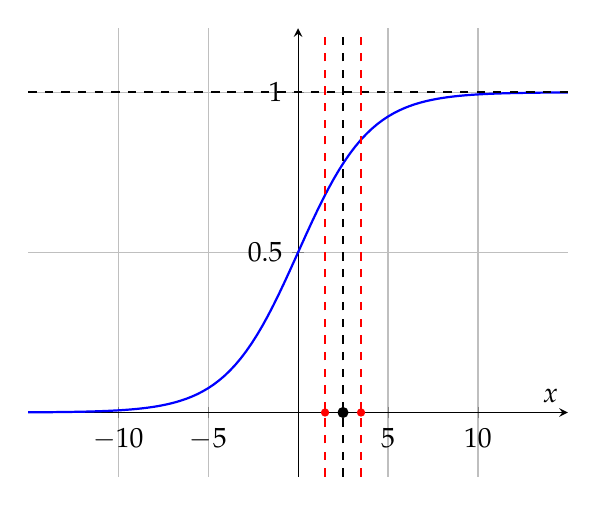
\begin{tikzpicture}
		\begin{axis}[
			axis lines=middle,
			xlabel=\(x\),
			yticklabel style={
				/pgf/number format/fixed,
				/pgf/number format/precision=1
			},
			ytick={0,0.5,1},
			xtick={-10,-5,0,5,10},
			grid,
			domain=-15:15,
			samples=100,
			ymax=1.2, % Adjusted y-axis to go a bit above 1
			ymin=-0.2
			]
			\addplot[blue,thick] {1/(1+exp(-0.5*x))};
			\addplot[dashed, black, thick] {1}; % Dashed horizontal line at y=1
			\fill [black] (axis cs:2.5,0) circle (2pt);
			\fill [red] (axis cs:1.5, 0) circle (1.5pt); 
			\fill [red] (axis cs:3.5, 0) circle (1.5pt); 
			\addplot[black, thin, dashed] coordinates {(2.5,-0.2) (2.5,1.2)};
			\addplot[red, thin, dashed] coordinates {(1.5,-0.2) (1.5,1.2)};
			\addplot[red, thin, dashed] coordinates {(3.5,-0.2) (3.5,1.2)};
		\end{axis}
	\end{tikzpicture}
	\caption{Illustration of the proposed model on a logistic function given by \Cref{eq:logit of X}. The black vertical line at $x=2.5$ denotes the mean presence of a metabolite in the system. Flanking this, the two red dashed lines depict potential shifts in this average presence due to the influence of covariates, denoted as $\epsilon_c$ in \Cref{eq:logit of X}.}
	\label{fig: example sigmoid function}
\end{figure}

In \Cref{fig: example sigmoid function}, a graphical representation illustrates the probabilistic association of a metabolite's presence within a particular species, predicated upon its mean prevalence across a taxonomic spectrum (denoted by the black vertical line at $x=2.5$). Consider, for example, a metabolite ubiquitously observed across various taxa. If a distinct clade within the phylogenetic tree conspicuously lacks this metabolite, the likelihood of its occurrence in species phylogenetically proximate to this clade diminishes — as indicated by the leftmost red line.
	
	\subsection{Emission probabilities}\label{subsec:emission probabilities}
	We consider several different types of data to inform about $\x$. This data may be of different dimensionality, e.g. may only discriminate along a subset of the axes or at a higher scale along some axes. For a particular data set $d=1, \ldots, D$, let $\bxi_d=\{\xi_{d1}, \ldots, \xi_{du}\}$ denote the sets of distinguished compartments. We then define the presence of ($\x(\xi_{du})=1$) or absence ($\x(\xi_{du})=0$) in set $\xi_{du}, u=1\ldots,U,$ as
	
	\begin{equation}
		\x(\xi_{du}) = \min \left(1, \sum_{c \in \xi_{du}} x_c \right).
	\end{equation}

	\subsection{Data sources}\label{subsec: data sources}
	We consider two sets of data informative about $\x$: i) Presence-absence data obtained with mass-spectrometry and ii) presence-only reports of specific metabolites in specific species.
	
	\subsubsection{Mass spectrometry}
	 Let $\bd _{sj}=(d_{sj1}, \ldots, d_{sjM})$ be the presence-absence vector of each metabolite $m$ obtained with mass-spectrometry run $j=1,\ldots,J_s$ performed on species $s$. Assuming a false-positive and false-negative error rates $\epsilon_{01}$ and $\epsilon_{10}$, respectively, we have
	
	\begin{equation}\label{eq:mass spec error rate}
		\P(\bd_{sj}|\x, \epsilon_{01}, \epsilon_{10}) = \prod_m \left[ x_{sm}\left(\epsilon_{10}^{1-d_{sjm}}(1-\epsilon_{10})^{d_{sjm}}\right) + (1-x_{sm})\left( \epsilon_{01}^{d_{sjm}}(1-\epsilon_{01})^{1-d_{sjm}}\right)\right]
	\end{equation}
	\subsubsection{LOTUS}
	
	As previously stated, LOTUS database \cite{rutzLOTUSInitiativeOpen2022} lists known occurrences of metabolites in species. Let $L_{ms} = 1$ denote a known occurrence of metabolite $m$ in species $s$, while $L_{ms}=0$ denotes that no evidence for such an occurrence has been reported, either because the metabolite $m$ is truly absent in species $s$ or because of a lack of research effort.
	
	Let us denote by $R_{sm}$ the probability of discovery of metabolite $m$ in species $s$ such that
	\begin{equation}\label{eq:prob lotus given x and Rsm}
		\P(L_{ms}|\x(\xi(m,s)), R_{ms}) = 
		\begin{cases}
			0 \quad &\mathrm{if\ } \x(\xi(m,s))=0 \mathrm{\ and\ } L_{ms} = 1,\\
			1 \quad &\mathrm{if\ } \x(\xi(m,s))=0 \mathrm{\ and\ } L_{ms} = 0,\\
			R_{ms} \quad &\mathrm{if\ } \x(\xi(m,s))=1 \mathrm{\ and\ } L_{ms} = 1,\\
			1- R_{ms} \quad &\mathrm{if\ } \x(\xi(m,s))=1 \mathrm{\ and\ } L_{ms} = 0,
		\end{cases}
	\end{equation}
	
	where $\xi(m,s)$ is the set of compartments relevant for metabolite $m$ and species $s$, i.e. all compartments $c$ for which $\tau_\M(c)=m$ and $\tau_S(c)=s$.
	
	To quantify the research effort $R_{ms}$ of a particular entry $L_{ms}$, we will rely on two measures, the total number of relevant papers published for metabolite $m$ ($P_m$) and for species $s$ ($Q_s$), such that
	
	\begin{equation}\label{eq:research effort}
		R_{ms} = 1 - e^{-\gamma P_m - \delta Q_s}
	\end{equation}
	
	with positives scalars $\gamma$ and $\delta$. In \Cref{fig:DAG naive model} we show a  Directed Acyclic Graph (DAG) of the proposed model. 
	
	\begin{figure}[h]
		\centering
		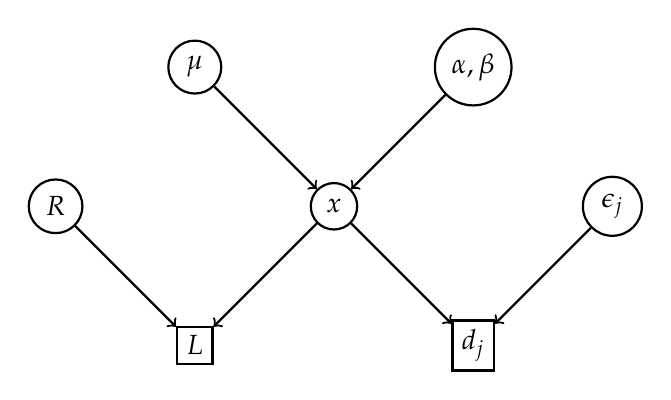
\begin{tikzpicture}[node distance={25mm}, thick, main/.style = {draw, circle}]
			\node[main] (1) {$\boldmath{x}$};
			\node[main] (2) [above left of=1] {$\mu$};
			\node[main] (3) [above right of=1] {$\alpha, \beta$};
			\node[draw] (4) [below right of=1] {$d_{j}$};
			\node[draw] (5) [below left of=1] {$L$};
			\node[main] (6) [above right of=4] {$\epsilon_j$};
			\node[main] (7) [above left of=5] {$R$};
			
			\draw[->] (2) -- (1);
			\draw[->] (3) -- (1);
			\draw[->] (1) -- (4);
			\draw[->] (1) -- (5);
			\draw[->] (6) -- (4);
			\draw[->] (7) -- (5);
		\end{tikzpicture}
		\caption{In the Directed Acyclic Graph (DAG) representing the \textit{naive model}, the variable $x$ denotes the binary state of a molecule's presence or absence within a designated species. Herein, $\mu$ signifies the mean presence along a specified axis. Both $\alpha$ and $\beta$ denote the axis-specific intercept and a positive scalar constant, respectively. The parameter $R$ stands for the dedicated research effort given to find $x$ while $L$ is indicative of the presence or absence of $x$ within the LOTUS database. The term $d_j$ characterizes the $j^{th}$ iteration of mass spectrometry executed for the particular species. Finally, $\epsilon_j$ quantifies the affiliated error rates, as elaborated in \Cref{eq:mass spec error rate}. }
		\label{fig:DAG naive model}
	\end{figure}


\section{Random Markov Field}\label{sec:methods:random markov field}

As previously stated, our objective is to infer the occurrence or absence of metabolites across a collection of samples, which are differentiated by discrete dimensions such as species, tissue type, and environmental conditions or any other arbitrary dimension. We hypothesize that the distribution pattern of these metabolites is moderated by shared characteristics within each dimension. For instance, metabolites can exhibit a similar distribution across phylogenetically close species, or if their synthesis pathways are interrelated. To quantitatively represent such similarities, we use a Markov random field approach \cite{sherringtonSolvableModelSpinGlass1975, kindermannMarkovRandomFields1980}.

Let $D$ denote the total number of dimensions. Without any loss of generality, we assume the first dimension corresponds to the metabolite. Each dimension, denoted by $d=1, \ldots, D$, consists of a set $\E_d$ of discrete entities (e.g., individual species along the species dimension). We model similarities between entries of dimension $d$ using a Markov process along a known tree $\T_d$ consisting of $\N_d = \E_d \cup \R_d \cup \I_d$ nodes, of which the entries $\E_d$ are leaves, connected to the set of roots $\R_d$ through a set $\I_d$ of internal nodes. We thus have $\E_d \cap \R_d = \varnothing$, $\E_d \cap \I_d = \varnothing$ and $\R_d \cap \I_d = \varnothing$. For every node $n \in \N_d, n \notin \R_d$ that is not a root, we denote $p(n) \in \N_d$ its parent node and $b(n) \geq 0$ the length of the branch connecting it to its parent.

We denote $\X$ a Markov Random Field of which each variable $x \in \X$ represents a unique combination of nodes from each dimension $D$, indicating the presence ($x=1$) or absence ($x=0$) of a metabolite. Let $\delta_d(x) \in \N_d$ reflect the node of $x$ in dimension $d$ with $\delta_1(x)$ indicating the metabolite of $x$, and let $\delta(x)=(\delta_1(x), \ldots, \delta_D(x))$. We only consider two sets of variables: 1) the set $\Y$ of variables representing an entry in each dimension such that for a variable $y\in\Y$, $\delta_d(y) \in \E_d$ for all $d=1, \ldots, D$, and 2) the set $\Z$ of variables representing leaves in all dimensions except one such that for a variable $z \in \Z$, $\delta_k(z) \in \I_k$ and $\delta_d(z) \in \E_d$ for all $d \neq k$. We then have $\X = \Y \cup \Z$ and $\Y \cap \Z = \varnothing$.

We suppose that the joint density of $\X$ can be factorized over a set of cliques $\Ccal$. Each clique $c \in \Ccal$ consist of a set of variables $x_1, x_2, \ldots \in \X$ that represent the same leaves in all but one dimension $k$. Specifically, for all $x \in c$, $\delta_d(x) \in \E_d$ for all $d \neq k$ and $\delta_k(x) \in \N_k$, and for all $x_i, x_j \in c$, $\delta_{-k}(x_i) = \delta_{-k}(x_j)$, where $\delta_{-k}(x)$ denotes the vector of nodes of $x$ in all dimensions but $k$. For such a clique, we will refer to the dimension $\nu(c) = k$ as its \emph{variable} dimension and will denote by $\delta_{-\nu(c)}(c)$ the vector of nodes in the \emph{fixed} dimensions. By definition, $\delta_{-\nu(c)}(c)=\delta_{-\nu(c)}(x)$ for every $x \in c$.

We will further denote by $\Ccal_k \subset \Ccal$ the subset of cliques that share the variable dimension $k$, i.e. $\nu(c)=k$ for all $c \in \Ccal_k$. Note that each clique is in exactly one subset ($\Ccal_k \cap \Ccal_d = \varnothing$ for all $k \neq d$) and cliques of the same subset do not share any variables ($c_1 \cap c_2 = \varnothing$ for all $c_1, c_2 \in C_k$). However, each variable $x \in \Y$ will be part of exactly one clique from each subset: the clique $c \in \Ccal_k$ for which $\delta_{-k}(c) = \delta_{-k}(x)$. In contrast, each variable $x \in \Z$ will be part of exactly one clique: the clique $c \in \Ccal$ for which $\delta_{-\nu(c)}(c) = \delta_{-\nu(c)}(x)$ and $\delta_{\nu(c)}(x) \in \I_{\nu(c)}$.

The joint density of $\X$ factorizes as
\begin{equation}
	\P(\X) = \prod_{d=1}^D \prod_{c \in \Ccal_d} \phi(c),
\end{equation}

where
we model the clique functions $\phi(c)$ using a Markov model along tree $\T_d$. Let

\begin{equation}
	\bLambda_c =
	\begin{pmatrix}
		-\mu_{c1} & \mu_{c1}\\
		\mu_{c0} & -\mu_{c0}\\
	\end{pmatrix}
\end{equation}

be the rate matrix for changes between states 0 and 1 along the tree. For each node $n \in \N_d, n \notin \R_d$ that is not a root, the transition probabilities between parent node $p(n)$ and $n$ are then given by

\begin{equation}
	\bP(n) = \exp(\bLambda_c b(n)).
\end{equation}

We assume the root state probabilities are given by the stationary distribution of the Markov chain:
\begin{equation}
	\bP_{\infty} = \left(\frac{\mu_{c0}}{\mu_{c0} + \mu_{c1}}, \frac{\mu_{c1}}{\mu_{c0} + \mu_{c1}}\right).
\end{equation}


The clique function $\phi(c)$
\begin{equation}
	\phi(c) = \prod_{x \in c, }\Big( \Ind(x \in \R_{\nu(c)})[\bP_{\infty}]_x + \Ind(x \notin \R_{\nu(c)}) [\bP(\delta_{\nu(c)}(x))]_{p_{c}(x), x} \Big)
\end{equation}

where we used the shorthand $x \in \R_{\nu(c)}$ for $\delta_{\nu(c)}(x) \in \R_{\nu(c)}$ to indicate whether the node in the variable dimension of $c$ of $x$ is a root and $p_{c}(x)$ to identify the variable $z \in c$ for which $\delta_{\nu(c)}(z) = p(\delta_{\nu(c)}(x))$.

\begin{figure}[h]
	\centering
	\begin{subfigure}[b]{0.49\textwidth}
		\centering
		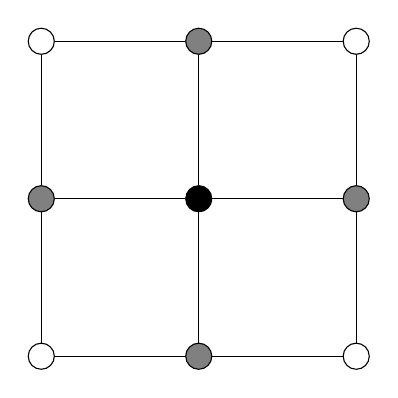
\begin{tikzpicture}[scale=2]
			% Define nodes
			\node[fill=black, circle, draw] (center) at (1,1) {}; % Central node
			\node[fill=gray, circle, draw] (top) at (1,2) {};     % Top node
			\node[fill=gray, circle, draw] (bottom) at (1,0) {};  % Bottom node
			\node[fill=gray, circle, draw] (left) at (0,1) {};   % Left node
			\node[fill=gray, circle, draw] (right) at (2,1) {};  % Right node
			\node[fill=white, circle, draw] (topleft) at (0,2) {};
			\node[fill=white, circle, draw] (topright) at (2,2) {};
			\node[fill=white, circle, draw] (bottomleft) at (0,0) {};
			\node[fill=white, circle, draw] (bottomright) at (2,0) {};
			
			% Connect nodes
			\draw (center) -- (top);
			\draw (center) -- (bottom);
			\draw (center) -- (left);
			\draw (center) -- (right);
			\draw (top) -- (topleft);
			\draw (top) -- (topright);
			\draw (bottom) -- (bottomleft);
			\draw (bottom) -- (bottomright);
			\draw (left) -- (topleft);
			\draw (left) -- (bottomleft);
			\draw (right) -- (topright);
			\draw (right) -- (bottomright);
		\end{tikzpicture}
		\caption{}
		\label{fig:Ising model}
	\end{subfigure}
	\hfill
	\begin{subfigure}[b]{0.49\textwidth}
		\centering
		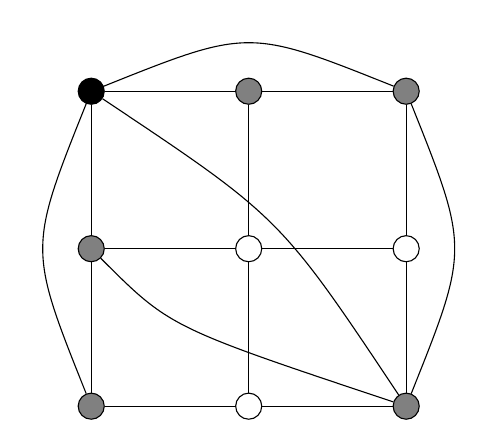
\begin{tikzpicture}[scale=2]
			% Define nodes
			\node[fill=white, circle, draw] (center) at (1,1) {};      % Central node
			\node[fill=gray, circle, draw] (top) at (1,2) {};         % Top node
			\node[fill=white, circle, draw] (bottom) at (1,0) {};      % Bottom node
			\node[fill=gray, circle, draw] (left) at (0,1) {};        % Left node
			\node[fill=white, circle, draw] (right) at (2,1) {};       % Right node
			\node[fill=black, circle, draw] (topleft) at (0,2) {};
			\node[fill=gray, circle, draw] (topright) at (2,2) {};
			\node[fill=gray, circle, draw] (bottomleft) at (0,0) {};
			\node[fill=gray, circle, draw] (bottomright) at (2,0) {};
			
			% Connect nodes with straight lines
			\draw (center) -- (top);
			\draw (center) -- (bottom);
			\draw (center) -- (left);
			\draw (center) -- (right);
			\draw (top) -- (topleft);
			\draw (top) -- (topright);
			\draw (bottom) -- (bottomleft);
			\draw (bottom) -- (bottomright);
			\draw (left) -- (topleft);
			\draw (left) -- (bottomleft);
			\draw (right) -- (topright);
			\draw (right) -- (bottomright);
			
			% Connect nodes with parabolic edges
			\draw (topleft) .. controls (-0.4,1) .. (bottomleft);
			\draw (topright) .. controls (2.4,1) .. (bottomright);
			\draw (topleft) .. controls (1.2, 1.2) .. (bottomright);
			\draw (topleft) .. controls (1, 2.4) .. (topright);
			\draw (left) .. controls (0.5, 0.5) .. (bottomright);
		\end{tikzpicture}
		\caption{}
		\label{fig: Ising model higher order}
	\end{subfigure}
	\caption{Representation of a Markov random field through an undirected graphical model where vertices depict arbitrary values and edges denote inter-nodes connectivity. \textbf{(a)} The Ising model \cite{isingBeitragZurTheorie1925} characterizes nearest-neighbour interactions. In this model, given the state of the grey nodes, the central black node becomes conditionally independent of all external nodes. \textbf{(b)} An \textit{advanced} structural representation, incorporating higher-order interactions beyond the traditional Ising model. Analogously in our proposed model, interactions extend beyond immediate neighbours, encompassing higher-order relationships as described by the trees $\T$. The illustration was conceptualized based on insights and frameworks derived from \cite{MarkovRandomField} and \cite{acarMarkovRandomField2016}. }
	\label{fig:MRF}
\end{figure}

In \Cref{fig:MRF}, a prototypical representation of a Markov Random Field is depicted. The Ising model, as illustrated in \Cref{fig:Ising model}, operates under the premise that a node's state is solely contingent upon its immediate neighbours. Contrarily, our proposed model, akin to the structure presented in \Cref{fig: Ising model higher order}, embodies intricate relationships reminiscent of phylogenetic interconnections. Within our framework, the state of a given node is not merely influenced by its proximal counterparts within the phylogeny, but also by the relational distances encompassing those neighbours.

\subsection{Data sources}\label{subsec:data source RMF}
The probabilities of the data given $x$ were formulated employing the same model as delineated in \Cref{subsec: data sources}.
\begin{figure}[h]
	\centering
	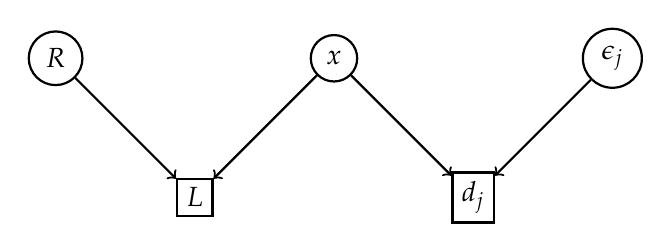
\begin{tikzpicture}[node distance={25mm}, thick, main/.style = {draw, circle}]
		\node[main] (1) {$\boldmath{x}$};
		\node[draw] (4) [below right of=1] {$d_{j}$};
		\node[draw] (5) [below left of=1] {$L$};
		\node[main] (6) [above right of=4] {$\epsilon_j$};
		\node[main] (7) [above left of=5] {$R$};
		
		\draw[->] (1) -- (4);
		\draw[->] (1) -- (5);
		\draw[->] (6) -- (4);
		\draw[->] (7) -- (5);
	\end{tikzpicture}
	\caption{In the Directed Acyclic Graph (DAG) for the RMF model, $x$ denotes the binary state of a molecule's presence or absence in a designated species. $R$ signifies the research effort allocated towards the determination of $x$. $L$ embodies the incidence of $x$ within the LOTUS database. The term $d_j$ is representative of the $j^{th}$ iteration of mass spectrometry performed on the specific species in question. Lastly, $\epsilon_j$ quantifies the associated error rates, as detailed in \Cref{eq:mass spec error rate}.}
	\label{fig:DAG_model}
\end{figure}
In \Cref{fig:DAG_model}, we illustrate the Directed Acyclic Graph (DAG) representation of the proposed model.


\section{Graph Convolution Neural Network (GraphSAGE)}\label{sec:theory:HinSAGE}
The low-dimensional representation of nodes within large graphs plays a critical role in various domains of scientific research and industrial applications, such as bioinformatics, social networks, and content recommendation systems. The utilization of these embeddings has proven effective in diverse prediction tasks, including clustering, node classification, and link prediction. However, traditional methods for generating these embeddings have predominantly focused on the transductive setting, requiring all nodes to be present during training and thus limiting generalization to unseen nodes or entirely new subgraphs \cite{groverNode2vecScalableFeature2016, perozziDeepWalkOnlineLearning2014}.

GraphSAGE (SAmple and aggreGatE) \cite{hamiltonInductiveRepresentationLearning2017} was presented as a solution to this challenge, offering a general inductive framework that leverages both node feature information and topological structure. Unlike transductive approaches, which rely on matrix factorization and are constrained to fixed graphs, GraphSAGE is designed to efficiently generate embeddings for previously unseen nodes.

The novelty of GraphSAGE lies in its ability to learn a function that generates embeddings through the sampling and aggregation of features from a node's local neighbourhood. It utilizes a set of trainable aggregator functions that encapsulate information from different search depths (hops), or away from a given node. By simultaneously learning the topological structure and distribution of node features in the neighbourhood, GraphSAGE accommodates feature-rich graphs as well as graphs lacking specific node features.

The applicability of GraphSAGE extends beyond simple convolutions, embracing a framework that generalizes Graph Convolutional Networks (GCNs) for the task of inductive unsupervised learning \cite{kipfSemiSupervisedClassificationGraph2016}. Unlike traditional methods that optimize embeddings for each node, GraphSAGE's inductive approach promotes efficiency and adaptability, allowing for a seamless alignment of newly observed subgraphs with pre-existing node embeddings.

GraphSAGE is particularly well-suited for the task of predicting which molecule is present in which species due to its robust inductive learning framework that generalizes to unseen nodes and subgraphs. In the context of biological data, such as molecular structures and species interactions, GraphSAGE's ability to leverage both the topological structure and node feature information offers a powerful means to understand the complex relationships within and across molecular graphs. Its novel approach of sampling and aggregating features from a node's local neighbourhood enables the capture of intricate patterns and structural properties that can be essential in identifying molecular presence across species. Furthermore, the inductive nature of GraphSAGE allows for the efficient generalization across different organisms, facilitating the prediction in entirely new or evolving graphs.

HinSAGE \cite{StellarGraphMachineLearning2018}, a derivative of GraphSAGE, has been specifically designed to handle heterogeneous graphs, where nodes and edges can be of various types. Developed by CSIRO's Data61, HinSAGE adeptly extends the foundational principles of GraphSAGE to contexts where the graph's heterogeneity introduces additional complexities. Unlike homogeneous graphs where the relation between nodes is more uniform, heterogeneous graphs present varying relationships and patterns, which HinSAGE is explicitly tailored to capture. By learning distinct embeddings for different types of nodes and relations, HinSAGE can uncover nuanced relationships within complex networks. This makes HinSAGE especially valuable for tasks such as predicting links within a bipartite graph, where one set of nodes represents species and another molecules. HinSAGE's capability to seamlessly navigate the intricacies of such heterogeneous structures ensures a richer and more accurate representation of the connections, fostering improved predictive accuracy for link prediction tasks in biological contexts where species-molecule interactions need to be discerned.

\chapter{Methods}\label{chap:Methods}
\section{Naive model}
Prior to the application of actual experimental data, a series of simulations were executed to evaluate the feasibility of estimating the entire set of parameters from the information contained within our dataset. Specifically, the variable $\mu$ was generated by sampling from a normal distribution with mean value of $0$ and variance of $1$. Meanwhile, the parameters $\alpha$, $\beta$, $\gamma$, and $\delta$ were each modelled using distinct exponential distributions, where individual values for the rate parameter $\lambda$ were attributed to each. In order to replicate the observed phenomenon, the number of papers per species $Q_s$ and per molecule $P_m$, were synthetically constructed by drawing from a Poisson distribution. Additionally, the variable $\sigma$ was simulated by drawing from a Wishart distribution \cite{wishartGENERALISEDPRODUCTMOMENT1928}.

As elaborated in \Cref{sec:methods:Naive approach}, the simulation process was initiated by drawing probabilities that $x=1$ from the \textit{expit} function, as defined in \Cref{eq:logit of X}. 
To emulate this binary characteristic, samples were subsequently drawn from a Bernoulli distribution, where the probability parameter was informed by the previous \textit{expit} function. Building upon this stochastic framework, the probabilities of LOTUS were constructed in accordance with \Cref{eq:prob lotus given x and Rsm,eq:research effort}. A  condition was imposed such that if $x$ for any given pair was $0$, then the corresponding probability was explicitly set to $0$.

These tailored probabilities were then employed as parameters for another Bernoulli distribution, generating binary outcomes that determined the number of papers associated with each pair. Specifically, if the result was $0$, the number of papers for that particular pair was set to $0$. Conversely, if the result was $1$, the number of papers for that pair was assigned based on random Poisson values that had been drawn previously in the simulation process.

This systematic approach resulted in the production of a simulated $x$ and a corresponding simulated LOTUS. This led to the occurrence of certain pairs that appearing empty, even though the molecule was indeed present within the species. All codes are available on \href{https://github.com/commons-research/anticipated-lotus}{GitHub}.
 
\section{Random Markov Field}
Due to time constraints of the thesis, test and simulation for this model were not performed. Code is available both on \href{https://bitbucket.org/wegmannlab/metabolite_inference/src/master/}{Bitbucket} and \href{https://github.com/anticipated-lotus/metabolite_inference}{GitHub}.

\section{HinSAGE}\label{sec:methods:HinSAGE}
The LOTUS database was aggregated to include only unique pairs of molecules and species. Once aggregated, the data was randomly partitioned into two subsets: 70\% allocated for training and 30\% for testing.

Graphs were systematically constructed for both the training and testing subsets using the software library NetworkX v3.1 \cite{SciPyProceedings_11}. In these graphs, individual nodes were designated to represent each molecule and species. When a specific species-molecule pair was identified in the LOTUS database, a directed edge was drawn between the two corresponding nodes. This procedure led to the creation of a bipartite graph, with directed edges labeled as "has" from species to molecules and "present in" from molecules to species.

The species' features were defined by extracting their phylogenetic information through the GBIF API \cite{GBIF, GbifPygbif2023}. Molecules' features were composed of their classification data from Classyfire \cite{djoumboufeunangClassyFireAutomatedChemical2016} and their Morgan Fingerprint \cite{rogersExtendedConnectivityFingerprints2010}, encoded using a 128-bit representation and a radius of 2.

In the preprocessing stage, features corresponding to both species characteristics and molecules' Classyfire properties were transformed through binary encoding. This transformation was essential to represent these categorical attributes as numerical values, thus making them suitable as features for the nodes within the graph. In the case of the molecules, two different sets of features, namely the binary-encoded Classyfire attributes and the Morgan Fingerprint, were concatenated to form a unified feature vector.

The model training was carried out using the Stellargraph library \cite{StellarGraphMachineLearning2018}. Two distinct models were trained to handle different relationships within the graph; one was tailored to the edges labeled "has" and the other to the edges described as "present in".

The HinSAGE models were configured with two layers, comprising 1024 neurons in each layer. The first layer was designed with a neighborhood sampling size of 3, enabling the model to encapsulate the local structural information, while the second layer utilized a sampling size of 1, thus focusing on immediate neighbors. By employing this hierarchical structure, the models could capture different scales of locality in the graph.

Furthermore, the HinSAGE models were implemented with a mean aggregator function, which served to combine the features of the neighboring nodes, thus generating a representative feature vector for each target node. A dropout rate of 0.3 was applied to mitigate the risk of overfitting, and "elu" and "selu" activation functions were utilized in the respective layers. These activation functions were chosen for their properties in mitigating vanishing gradient problems, thereby aiding the convergence of the model during the training process. 

We moved forward with an objective to predict the entire scope of the LOTUS database, specifically targeting the probability for every possible species-molecule combination. This analysis covered a total of $5.45 \cdot 10^9$ pairs. All codes are available on \href{https://github.com/anticipated-lotus/GNN}{Github}.


\chapter{Results and Discussion}
\section{Naive approach}
In the preliminary stages of our research, we recognized the necessity to understand the behaviour of our model prior to applying it to the actual dataset. To achieve this, we carried out a series of simulations to assess if the model's parameters could be accurately estimated based on these synthetic data.

Specifically, we simulated 100 molecules and 10 species in alignment with the theoretical framework described by Equations \ref{eq:prob lotus given x and Rsm} and \ref{eq:research effort}.

For the parameter estimation process, we employed Markov Chain Monte Carlo (MCMC) techniques to accurately estimate the parameters $\gamma$ and $\delta$. The results of this estimation process were consistent and close to our simulated values, demonstrating the effectiveness of the approach.

Furthermore, we utilized Gibbs sampling to estimate the variable $x$. This method too yielded satisfactory results, corroborating the validity of our model in this aspect.

However, the challenges encountered during the modelling and simulation process were primarily centred around the convergence of the axis-specific intercepts $\mu$. This crucial component, detailed in Equation \ref{eq:logit of X}, resisted precise estimation through our initially chosen techniques. During this period of reevaluation, the proposition of interpreting our data as a graph surfaced, adding a new dimension to our perspective. Persisting with our original data treatment no longer seemed intuitive. Given the inherent structure and relationships in our dataset, transitioning to a graph-based approach felt more logical and natural. As a result, the inability to accurately estimate $\mu$ and the allure of a graph-centric methodology prompted us to explore alternative models and techniques, seeking a better alignment with the intrinsic characteristics of our data. To reproduce our simulations, codes are available on \href{https://github.com/commons-research/anticipated-lotus}{GitHub}.

\section{Random Markov Field}
Due to time constraints of the thesis, test and simulation for this model were not performed. However this could work since paper TODO 

\section{Graph Neural Network}
Using unseen edge data to assess the models, the performance measures showed that each model had varying degrees of accuracy. Particularly, the 0.92 accuracy was demonstrated by the model that was trained to predict the "present in" relationships. The model that attempted to predict the "has" associations, in contrast, had an accuracy of 0.8.

It is significant to note that a probability value of 0.5 was used as the cutoff for assessing whether metabolites were present or absent. As a result, probability above this cutoff were classed as a presence, denoted as $x=1$, and values below this cutoff were classified as an absence, denoted by $x=0$.

\begin{figure}[h]
	\centering
	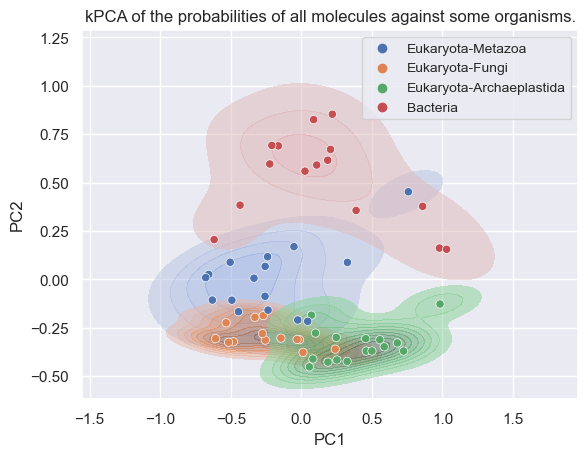
\includegraphics[scale=0.7]{figure/kPCA}
	\caption{kPCA visualization of sampled species across primary biological domains. The second principal component distinguishes between domains, with potential influences from our GNN's molecular pattern recognition or biases within the LOTUS database.}
	\label{fig:kPCA}
\end{figure}

After predicting the entirety of the LOTUS database, we randomly sampled a dozen species from each primary biological domain, excluding Archaea. Each of these species was associated with $148'190$ probability values. A kernel Principal Component Analysis (kPCA) was then carried out to identify potential variance between the domains. Kernel Principal Component Analysis (kPCA), as opposed to classic Principal Component Analysis (PCA), became the preferred approach given the high-dimensionality of our dataset. The advantages of kPCA over PCA are its skill at handling large data dimensions and its ability to recognise non-linear correlations between features that PCA's linear assumptions might miss. This innate ability makes sure that kPCA keeps the most important and complex relationships within the data as well as reducing the dimensions of the data.

A definite distinction between the biological domains can be seen by looking at \Cref{fig:kPCA}. To explain these observed variances, two hypotheses have been put forth. First, by accurately portraying the molecular signatures unique to each domain, our Graph Neural Network (GNN) may be skilled at differentiating between them. Alternately, it is possible that the kPCA is mostly displaying the chemical biases included in the LOTUS database. Given that the LOTUS database organises its data according to triples of molecules-species-papers, it is reasonable to think that a preponderance of extensively researched molecules, meriting scholarly publication, are intrinsically specific to particular domains i.e are specialized metabolites. This claim is supported by \textit{Rutz et al.} \cite{rutzLOTUSInitiativeOpen2022}, who note that a significant majority (more than 90\%) of the compounds included in LOTUS display domain specificity. The patterns in the kPCA results that have been found may be explained by such innate biases. Either of the previous assumptions has to be supported by a more in-depth examination.
 
\begin{figure}[h]
	\centering
	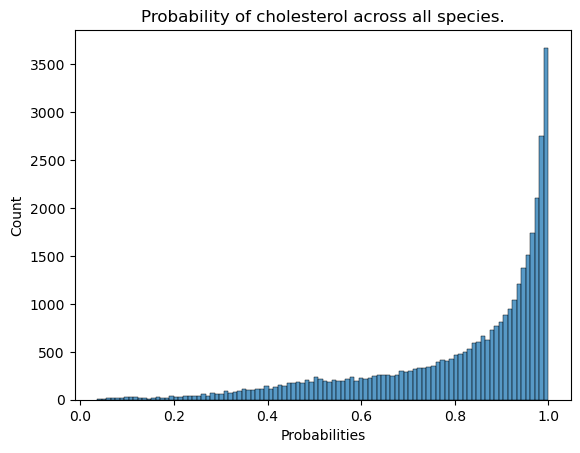
\includegraphics[scale=0.7]{figure/cholesterol}
	\caption{Probability distribution of cholesterol presence across species in the LOTUS database. The species already associated with cholesterol were removed before the calculations.}
	\label{fig: hist cholesterol}
\end{figure}

In \Cref{fig: hist cholesterol,fig: hist erythromycin}, we present the probability distributions of cholesterol and erythromycin presence across the species present in LOTUS. Based on the literature \cite{o2013merck, international1979iarc}, cholesterol is ubiquitously found. The predictions of our algorithm align with this notion, indicating a prevalent cholesterol presence in most species. This predictive consistency is attributed to the mechanics of GraphSAGE. Given that cholesterol is associated with a significant 522 species in the LOTUS database, the algorithm effectively capitalizes on this trend to offer insightful predictions.

Conversely, erythromycin's representation in the database is comparatively limited, being connected to merely eight species. Notably, these connections predominantly pertain to bacteria from the Actinobacteria phylum. As a result, our model tends to predict a restricted occurrence of erythromycin across species, as visualized in \Cref{fig: hist erythromycin}. Yet, when it anticipates its presence, the accuracy is commendable. Key genera such as Streptomyces are correctly identified, with minor discrepancies like Micromonospora, as detailed in \Cref{table: Erythromycin top scores}. This showcases the GraphSAGE's capability in discerning potential associations between molecules and species, even in scenarios of sparse data. 

\begin{figure}[h]
	\centering
	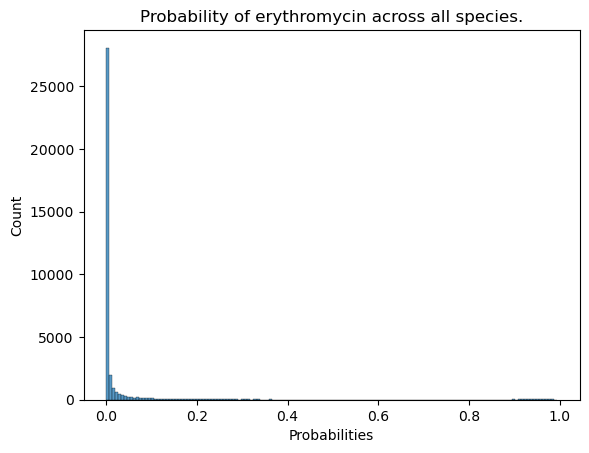
\includegraphics[scale=0.7]{figure/erythromycin}
	\caption{Probability distribution of erythromycin presence across species in the LOTUS database. The species already associated with erythromycin were removed before the calculations.}
	\label{fig: hist erythromycin}
\end{figure}

While GraphSAGE has demonstrated a commendable capability in making nuanced predictions, its proficiency in discerning the occurrence of molecules in species is not without boundaries. For instance, delving into the case of \textit{Streptomyces diastaticus} presented in \Cref{table: Erythromycin top scores}, a glaring lack of documentation regarding its erythromycin production exists in the contemporary literature. An exception lies in the findings of \cite{graham23SRibosomalRibonucleic1979}, which propose that \textit{Streptomyces diastaticus} might indeed exhibit sensitivity to erythromycin. A similar ambiguity surrounds \textit{Streptomyces drozdowiczii}, with no documented evidence supporting the presence of erythromycin. Contrastingly, the potential presence of this molecule in \textit{Streptomyces achromogenes} is insinuated in the research presented by \cite{moosawiComputationalPredictionProperties2010}.

A thorough analysis using mass spectrometry of the highlighted species becomes necessary to confirm the reliability and effectiveness of our approach. This could reveal new molecular species relationships and provide empirical support for the hypothesised associations presented in \Cref{table: Erythromycin top scores}.

\begin{table}[h]
	\centering
	\caption{Erythromycin was originally discovered in \textit{Saccharopolyspora erythraea } \cite{beranIsolationErythromycinNoxide1991}. Here we show the top 10 species that could contain erythromycin and that are not present in LOTUS.}
	\begin{tabular}{lr}
		\toprule
		Species & Probability \\
		\midrule
		Streptomyces diastaticus & 0.9944 \\
		Streptomyces drozdowiczii & 0.9939 \\
		Streptomyces antibioticus & 0.9928 \\
		Micromonospora & 0.9927 \\
		Streptomyces achromogenes & 0.9924 \\
		Streptomyces griseus & 0.9919 \\
		Streptomyces griseosporeus & 0.9912 \\
		Streptomyces albogriseolus & 0.9906 \\
		Streptomyces varsoviensis & 0.9899 \\
		Streptomyces ansochromogenes & 0.9898 \\
		\bottomrule
	\end{tabular}
	\label{table: Erythromycin top scores}
\end{table}

An inherent bias in favour of specialised metabolites represents another important constraint. Understanding the existence of basic metabolites like water frequently does not attract academic curiosity. Predictions are then difficult since the research output rarely associates such a chemical with its related species. This is demonstrated by the LOTUS database, which only records six instances of water, leading to poor predicative results as seen in \Cref{fig: water probabilities}.

Additional complexities exist that limit the effectiveness of our model. In the training stage of GraphSAGE, the algorithm only samples negative edges from edges that don't exist in the graph.This methodology could introduce potential anomalies; certain molecules may in fact be associated with distinct species, but the algorithm is predisposed to miss such associations. The algorithm's indifference for phylogenetic distances is a serious matter as well. Although evolutionary information is encoded in the node properties, the larger structural architecture lacks it, which unintentionally leaves out important information. This shortcoming might affect the precision of inferring occurrences in particular phylogenies. 

\begin{figure}[h]
	\centering
	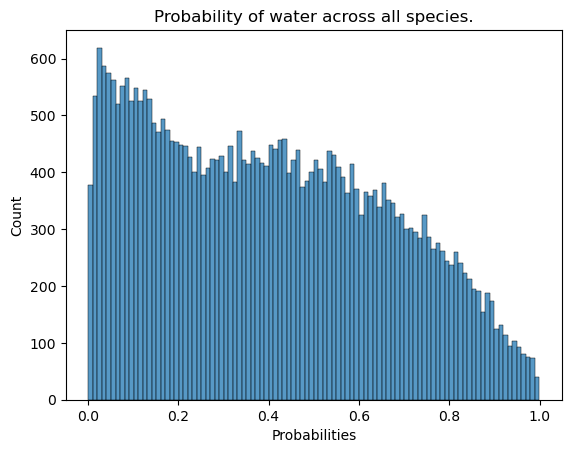
\includegraphics[scale=0.7]{figure/water}
	\caption{Probability distribution of water across species in the LOTUS database. The species already associated with water were removed before the calculations. This visualization sheds light on a limitation of our model. It's a reasonable expectation that water is a ubiquitous component in a vast majority of species. However, with only six water mentions in LOTUS, our predictions seem to fall short. Integrating mass spectrometry data within the model could mitigate this problem such discrepancies.}
	\label{fig: water probabilities}
\end{figure}

Lastly, the current model configuration does not factor in the research effort, as delineated in \Cref{eq:prob lotus given x and Rsm}. This omission could lead to biases, potentially comparing molecules with considerable documentation in a given species to ones with less characterization in a relatively unknown species.


\chapter{Conclusion and Future Work}
In the course of our research, we have demonstrated the feasibility of devising a model to predict the chemical compositions of organisms spanning the tree of life. By employing a framework that perceives phylogenies and molecules as graphs, we have been able to make superior predictions compared to rudimentary models.

The application of a Graph Neural Network (GNN) employing the GraphSAGE technique has proven effective as an initial strategy. Notably, this rudimentary implementation already yields reliable results for well-characterized metabolites. Nonetheless, several challenges emerged. Foremost among these is the technical issue of overlooking phylogenetic distances, which consequently diminishes the amount of available data. Additionally, the methodology employed for encoding molecular features, specifically the straightforward concatenation of Classyfire classification and Morgan fingerprint, may not be the ideal representation of the molecule's information.

A significant constraint of the GNN is its inability to augment the density of a graph. Given the notable sparsity of the edges, the GNN, based solely on the existing data, cannot enhance graph density. This characteristic is intrinsic to graph completion; hence the conventional recommendation is to commence training neural networks on densely populated regions of a graph.

From this arises a dichotomy of objectives: are we attempting to predict LOTUS, or are we genuinely aiming to discern the actual presence and absence of molecules throughout the tree of life? Our current GNN, we contend, addresses the former query. However, given the reasons highlighted earlier, particularly the intrinsic graph sparsity, this might not be the most pivotal question. Simply extrapolating LOTUS using this methodology would lead to predictions of manifestly extant edges without furnishing deeper insights. While augmenting the data in LOTUS or incorporating mass spectrometry data could offer potential solutions, they pose their own set of challenges, such as edge weighting and data integration.

Contrastingly, given that both GNN and Markov Random Field (MRF) address analogous issues \cite{jiaGraphBeliefPropagation2021}, our hypothesis is that MRF could yield more robust outcomes. The inherent flexibility of MRF, allowing for multi-dimensional data integration, could potentially ameliorate the molecule encoding challenge we encountered with GNN. Envisioning a model that integrates species phylogenies, the existing Classyfire classification tree structure, and a tree for the Morgan fingerprint could be transformative. However, one anticipated hurdle is the designation of accurate distances within the molecular tree. Furthermore, the proposed MRF model could seamlessly incorporate mass spectrometry data, a task currently beyond the capabilities of the GNN. Crucially, within this MRF model, both LOTUS data and mass spectrometry data would be treated as noisy observations rather than absolute truths, which is a major deviation from the GNN approach.

To conclude, our assertion is that further exploration and refinement of the MRF model could usher in significant advancements in metabolomics, ecology, and drug discovery. It is our aspiration that this research serves as a pioneering endeavor in this burgeoning domain of study.




\newpage
Through this work we have shown that it is possible to create a model for predicting the chemical composition of organisms across the tree of life. Our experiment showed that utilizing the natural way of thinking of phylogenies and molecules as graphs could allow for better predictions that a simple model. 

The GNN approach using GraphSAGE allowed for a good first approach. This simple implementation can already give sensible results for well established metabolites. However many problems arise. First some technical problems arise. Indeed, phylogenetic distances were not taken into account. This reduces the information that we have available. Secondly, the encoding of the features of molecules might not be optimal. Indeed, the simple concatenation of Classyfire classification and Morgan fingerprint might not be the optimal way to encode information of the molecule. 

Also, the GNN will not be able to densify a graph. Indeed, if the edges are very sparse (which is the case), the GNN will not be able to increase the density of the graph only by having been train on the current data. This is an inherent feature of graph completion and that is why is usually recommended to have highly dense regions on a graph and train the neural network on them to then complete the rest of the graph. 

Two questions arise from these problems. Are we trying to anticipate LOTUS ? Or are we trying to determine the true presence AND absence of molecules across the tree of life ? 

We believe, our current GNN is able to answer the first question however we don't believe that this first question is the most interesting one due to the argument made above about the sparsity of the graph. Indeed, anticipating LOTUS using this technique will result in anticipating the OBVIOUS possible existing edges but won't provide any more information. One could argue by updating LOTUS i.e. increasing the amount of information could densify the graph but that would be still to slow due to the immense sparsity of LOTUS. One could also argue to include mass spectrometry data but this would then require to weigh edges coming from MS and edges from LOTUS. Furthermore since the GNN is trains negatives edges on none existing edges, it is only able to predict the presence and not the absence of a pair. 

In contrast, since both GNN and Markov Random field are both approaches to a same problem \cite{jiaGraphBeliefPropagation2021}, we believe that our MRF could lead to significantly better results. Indeed, the model can take into account as many dimensions as it wants. This means that it could solve the previous problem of concatenation of features in the molecules. In fact, one could imagine the model containing three trees : the species phylogenies, the tree-like structure of the Classyfire classification (already exists) and a tree for the Morgan fingerprint were the molecules have been classified using Neighbour-Joining or Unweighted Pair Group Method with Arithmetic Mean (UPGMA). One problem could arise however: each branch in the tree should have a distance. This is trivial for species, but it might be more difficult to imagine for molecules. This model could also take into account the research effort (as stated in \Cref{subsec:data source RMF}). The model would also be able to integrate easily mass spectrometry data, thing that the GNN is not able to do yet. Moreover, in this model we treat LOTUS data and mass spectrometry data as noisy observation of $\X$ whereas in the GNN we consider them as a ground truth (which is a strong assumption that could lead to problems). 

In short, we believe that is worth spending time developing the MRF and this could lead to great advances in the world of metabolomics, ecology and drug discovery. We hope that this work was able to set the first mile stone in this field of research. 


\newpage
Question 1 : Do you want LOTUS anticipated ? 

Question 2 : Do you want the true presence/absence ?


Future work : Continue developing RMF. As shown in paper \cite{jiaGraphBeliefPropagation2021}, both model can work. Restart HinSAGE and include all phylogenies. Include mass spectrometry runs in all models. Knowledge graph completion. Add more data coming from knowledge graph completion. explain what it is. Insist on continuing on MRF since it has great potential. 

\section{Knowledge Graph Completion}
Knowledge Graphs (KGs) provide a robust technique for the consolidation of diverse data and the modelling of complex interactions, crucial for areas like forecasting the natural products present in various species \cite{ehrlingerDefinitionKnowledgeGraphs2016}. 

In its simplest form, a graph is a data structure that designates items (or "nodes") and the links (or "edges") between them. In the context of our discussion, nodes might symbolize different species, while edges could denote a variety of relationships such as common ecosystems, shared characteristics, or the potential to yield similar natural products. Depending on the kind of the relationships, the graph can either be directed (representing asymmetric relations) or undirected (symbolizing symmetric relations).

Two primary categories of graphs exist: homogeneous and heterogeneous. A homogeneous graph possesses nodes and edges of the same category. In this scenario, a homogeneous graph might be comprised of species nodes interconnected by edges representing a particular connection, like a mutual ecosystem. Conversely, a heterogeneous graph contains nodes and edges of diverse types. For instance, a heterogeneous graph in this case could encompass nodes representing species, ecosystems, and natural products, linked through various relationships like "inhabits", "generates", or "has common traits with".

A specific kind of graph known as multigraphs permits multiple edges between the same pair of nodes and can also accommodate loops. This is advantageous when there are various types of relations between the same pair of nodes. Multigraphs are predominantly heterogeneous.

A Knowledge Graph (KG) is a distinct type of graph used to encode significant knowledge concerning a specific domain. It is a directed, heterogeneous multigraph with domain-specific semantics for its node and relation types. In this setting, a KG could be employed to encode knowledge about species and their capability to produce natural products. The nodes in the KG, also known as entities, could symbolize different species, ecosystems, or specific natural products. The directed edges, usually represented as triples (head, relation, tail), encapsulate the relationships between these entities.

Knowledge graph embeddings are techniques to convert the discrete entities and relations in a KG into continuous vectors in a high-dimensional space, while preserving the original relationships from the KG \cite{wangKnowledgeGraphEmbedding2017}. This conversion to a continuous vector space is especially valuable in predicting missing information, like forecasting a species' potential to produce a specific natural product based on its relations with other entities in the KG.

In conclusion, KGs and their corresponding embeddings act as an essential instrument for encoding and analysing multifaceted, relational data. Within the context of predicting natural products in species, they can encapsulate and represent complex relationships between species, ecosystems, and the natural products themselves, potentially contributing to the discovery and comprehension of new natural products.

%----------------------------------------------------------------------------------------
%	THESIS CONTENT - APPENDICES
%----------------------------------------------------------------------------------------

\appendix % Cue to tell LaTeX that the following "chapters" are Appendices

% Include the appendices of the thesis as separate files from the Appendices folder
% Uncomment the lines as you write the Appendices

%\include{Appendices/AppendixA}
%\include{Appendices/AppendixB}
%\include{Appendices/AppendixC}

%----------------------------------------------------------------------------------------
%	BIBLIOGRAPHY
%----------------------------------------------------------------------------------------
%\printbibliography
\renewcommand{\bibname}{References}
\bibliographystyle{unsrturl}
\bibliography{/Users/Marco/BibTex/MyBibTex}


%----------------------------------------------------------------------------------------

\end{document}  
